% ch05 译文：原文第 4 节 4a（main.tex 第 1055–1190 行）
% [原文 p.20]
\section{离散商的 Fukaya 范畴\label{sec:Fukaya-category-discrete-quotient}}
设 $X$ 为 Weinstein 扇形，$G$ 为离散群，$G\curvearrowright X$ 为 $G$ 在 $X$ 上的作用；该作用精确辛、连续并且自由。我们进一步假设作用是 \emph{柱状的}（cylindrical），即：在 $X$ 的某个柱状端 $\partial_{\infty}X\times [0,+\infty)\hookrightarrow X$ 中，$X$ 上的 $G$-作用保持柱状坐标 $[0,+\infty)$，并且在无穷远边界 $\partial_{\infty} X$ 的每个接触边界上都是接触同胚。\par

由假设，商空间 $X/G$ 仍是 Weinstein 扇形，其无穷远理想边界为 $\partial_{\infty} X/G$。本节将用 $X$ 的包裹 Fukaya 范畴 $\mathcal{W} (X)$ 计算 $X/G$ 的包裹 Fukaya 范畴 $\mathcal{W} (X/G)$。本节的主定理是：

\begin{thm}[商的包裹 Fukaya 范畴]\label{thm:wrapped-Fukaya-quotient}
    存在 $A_{\infty}$-范畴的等价
    \[
        \mathcal{W} (X/G)\simeq\mathcal{W} (X)/G \simeq\mathcal{W}(X)_G
    \]
    它在取扭完成（twisted completion）之后成立，其中 $\mathcal{W} (X)/G$ 是 Fan--Keller--Qiu \cite{FKQ24} 发展的 dg 轨道范畴的 $A_{\infty}$-变体，而 $\mathcal{W}(X)_G$ 是 $\mathcal{W}(X)$ 关于 $G$-作用的同伦商；后者与 $\mathcal{W}(X)/G$ 的等价由 Christ \cite{Christ26} 证明。
\end{thm}

\begin{conceptbox}{轨道范畴（orbit category）}
给定范畴 $\mathcal{C}$ 与自同构 $F$，轨道范畴 $\mathcal{C}/F$ 的\textbf{对象仍与 $\mathcal{C}$ 相同}（并不取 $F$-轨道），态射则取成所有 $F^n$ 作用之后的直和 $\hom_{\mathcal{C}/F}(X,Y)=\bigoplus_{n\in\mathbb{Z}}\hom_{\mathcal{C}}(X,F^nY)$，复合带一个由幂次给出的扭。三角版本与导出版本要把直和换成直和补全，即只取有限和。本节用它描述「商掉群作用」的 A 侧：定理 \ref{thm:wrapped-Fukaya-quotient} 断言，$\mathcal{W}(X)/G$ 与真正的商空间 $X/G$ 的包裹 Fukaya 范畴在扭完成之后一致。
\par\smallskip\noindent{\footnotesize 参考：Keller, \emph{On triangulated orbit categories}, arXiv:math/0610212；Fan--Keller--Qiu \cite{FKQ24}。}
\end{conceptbox}

\begin{yizhu}[两种商不是一回事]
定理中的 $\mathcal{W} (X)/G$ 与 $\mathcal{W}(X)_G$ 是两个不同的商：前者是轨道范畴，把对象按 $G$-轨道等同、把态射取成所有群元素作用后的直和；后者是 $G$ 作用在同伦意义下的商（同伦商）。二者并不天然相等，等价只在扭完成之后成立，因此不能把它当作范畴层面的恒等。$A_{\infty}$-层面的等价还要在取同伦范畴之后才落到通常范畴上。
\end{yizhu}

\subsection{带群作用的 Weinstein 扇形}
本节回顾 Weinstein 扇形的定义，并在带有限生成离散群作用的 Weinstein 扇形上构造对该作用不变的 Weinstein 结构。回顾如下定义。

\begin{dfn}\label{defn:Liouville-sector-inf}
    \emph{Liouville 扇形}是一个三元组 $(X,\omega,Z)$：其中 $(X,\omega)$ 是带边辛流形，$Z$ 是 $X$ 上的完全向量场，且满足
    \begin{enumerate}[label=(\roman*)]
        \item （无限型）存在穷竭 $X=\displaystyle\bigcup_i X_i$，其中 $X_0\subseteq X_1\subseteq\dotsb$ 是一列紧的带角辛流形，使得对一切 $i$，$Z$ 沿 $\partial X_i\setminus\partial X$ 外指。
        \item 有 $\mathcal{L}_Z\omega =\omega$，即 $Z$ 以指数方式伸缩 $\omega$。
        \item 存在光滑函数 $I\colon\Nbd (\partial X)\to\mathbb{R}$（定义在 $\partial X$ 的某个开邻域上）、常数 $0<\alpha\leq 1$，以及对每个 $i$ 的紧子集 $K_i\subseteq\partial X\cap (X_i\setminus X_{i-1})$，使得在 $\displaystyle\bigcup_i K_i$ 之外有 $ZI=\alpha I$，并且 Hamilton 向量场 $X_I$ 沿 $\partial X$ 外指。
    \end{enumerate}
    若存在光滑函数 $\phi\colon X\to\mathbb{R}$，使得 $Z$ 关于 $\phi$ 是类梯度的、$\phi(\partial X_i)=\{r_i\}$ 是一列趋于 $\infty$ 的常数，并且 $\phi$ 在 $I^{-1}(0)$ 上的限制对某个取定的光滑函数 $I$ 定义了 Weinstein 结构，则称 $X$ 是 \emph{Weinstein} 的。
\end{dfn}

这个定义与 Ganatra--Pardon--Shende \cite{GPS20} 的原始定义相比，差别在于我们允许无限型的 Liouville 扇形；当 $\partial X=\emptyset$ 时，它与 \cite{CE12} 中的定义一致。

\begin{dfn}\label{defn:G-invariant-Weinstein-sector}
    设 $G$ 为 Lie 群，$(X,Z_X,\omega_X)$ 为 Liouville 扇形。若对每个 $g\in G$ 都存在 $f_g\in C^{\infty} (X;\mathbb{R})$（且光滑依赖于 $G$），使得 $g^{\ast}\lambda_X =\lambda_X +df_g$，并且 $\lambda_X +df_g$ 的零点落在 $X$ 的紧子集中，则称 $G$-作用 $G\curvearrowright X$ 是 \emph{精确辛}的。若对每个 $g\in G$ 都存在紧子集 $K_g\subseteq X$，使得 $g$ 在 $K_g$ 之外为恒等，则称该作用 \emph{紧支撑}。\par
    若对一切 $g\in G$ 都有 $g^{\ast}\lambda_X =\lambda_X$，其中 $\lambda_X$ 是 $Z_X$ 的辛对偶，则称 $X$ 上的精确辛 $G$-作用是 \emph{Liouville} 的。若 $X$ 进一步是 Weinstein 的、Weinstein 结构为 $\phi_X$，并且对一切 $g\in G$ 有 $g^{\ast}\phi_X =\phi_X$，则称该 $G$-作用是 \emph{Weinstein} 的。
\end{dfn}

\begin{lmm}
    设 $X$ 是 Weinstein 扇形，带有紧支撑的精确辛 $G$-作用，且 $G$ 为有限群，则 $X$ 上存在一个 Weinstein 结构，使得 $G$ 的作用成为 Weinstein 作用。
\end{lmm}

\begin{proof}
    \textbf{第一步.} 在每种情形下，我们都可以对每个 $g\in G$ 取光滑函数 $f_g\in C^{\infty} (X,\mathbb{R})$，使得 $g^{\ast}\lambda_X =\lambda_X +df_g$。我们要找 Liouville $1$-形式 $\lambda\coloneqq\lambda_X +df$，其中 $f\in C^{\infty}(X,\mathbb{R})$，使得对一切 $g\in G$ 有 $g^{\ast}\lambda =\lambda$。把 $g$ 代入即得
\[
        g^{\ast}\lambda -\lambda =d(f_g +f\circ g-f),
    \]
    因此 $f$ 应当满足恒等式
\begin{equation}\label{eq:invariance-condition}
        f_g +f\circ g-f=0
    \end{equation}
    对一切 $g\in G$ 成立。注意对 $h\in G$，有复合
\[
        h^{\ast}g^{\ast}\lambda_X =h^{\ast} (\lambda_X +df_g)=\lambda_X +d(f_h +f_g\circ h)=\lambda_X +df_{gh},
    \]
    故函数族 $\{f_g\}_{g\in G}$ 必须满足 $f_{gh}=f_h +f_g\circ h$（允许相差一个常数），而我们可以安排得使严格的恒等式在两种情形下都成立。\par
    \textbf{第二步.} 设 $G$ 有限，考虑函数
\[
        f=\frac{1}{\vert G\vert}\sum_{g\in G} f_g.
    \]
    不难验证对任意 $g\in G$，方程 \eqref{eq:invariance-condition} 都成立；因此 $1$-形式 $\lambda_G\coloneqq\lambda_X +df$ 满足 $d\lambda_G =\omega_X$ 与 $g^{\ast}\lambda_G =\lambda_G$。其对偶向量场为
\[
        Z_G =Z_X +X_f =Z_X+\frac{1}{\vert G\vert}\sum_{g\in G} X_{f_g},
    \]
    它是完全的，因为每个 $X_{f_g}$ 都在 $X$ 的某个给定紧子集之外为零。
\end{proof}

% [原文 p.22]
假设 $(X,Z,\omega)$ 是 \emph{有限型}的，即 $Z$ 的零点集紧。此时 Ganatra--Pardon--Shende 在 \cite{GPS20} 中构造了 $X$ 的 $A_{\infty}$-范畴 $\mathcal{W} (X,\lambda ,Z)$，称为 $X$ 的 \emph{包裹 Fukaya 范畴}。在 \cite{GPS24S} 中，他们进一步证明了

\begin{thm}[Viterbo 限制]\label{thm:Viterbo-restriction}
    设 $X_1, X_2$ 为有限型的 Weinstein 扇形，并设 $\bar{X}_1$（即 $X_1$ 中包含 $Z_1$ 全部临界点的紧带角辛子流形，且 $Z_1$ 沿 $\partial\bar{X}_1\setminus (\bar{X}_1\cap\partial X_1)$ 外指）可经辛嵌入映入 $X_2$，该嵌入把 $\partial X_1\cap\bar{X}_1$ 映入 $\partial X_2$，并使补集 $\overline{\bar{X}_2\setminus\bar{X}_1}$ 成为 Weinstein 配边；则存在本质满的 $A_{\infty}$-函子 $\mathcal{W} (X_2)\to\mathcal{W} (X_1)$，称为 \emph{Viterbo 限制}。
\end{thm}

\begin{conceptbox}{Viterbo 限制（Viterbo restriction）}
Viterbo 限制是包裹 Fukaya 范畴沿辛嵌入的「拉回」：当小扇形 $X_1$ 嵌在大扇形 $X_2$ 中、补集又是 Weinstein 配边时，$X_2$ 中的 Lagrangian 可以限制到 $X_1$，其包裹 Floer 上同调随之比较，于是得到函子 $\mathcal{W}(X_2)\to\mathcal{W}(X_1)$。它本质满，意思是 $X_1$ 的每个对象都已出现在 $X_2$ 中，只可能相差同构。本文用它把无限型扇形的范畴定义为有限型穷竭上的同伦极限：每一层的对象都由上一层经限制得到。
\par\smallskip\noindent{\footnotesize 参考：Ganatra--Pardon--Shende \cite{GPS24S}。}
\end{conceptbox}

\begin{yizhu}[限制的方向]
Viterbo 限制虽然名字叫「限制」，函子方向却是从大扇形到小扇形：$\mathcal{W} (X_2)\to\mathcal{W} (X_1)$，与平常上同调沿开子集限制的方向一致。本质满保证小扇形中的对象都能在未取极限之前被看到，这正是下一则定义中「用有限型穷竭取同伦极限」可行的依据。若把方向记反，就会误以为所有小扇形的范畴都嵌进大扇形的范畴，那是错的。
\end{yizhu}

利用这一点，以及给定一般 Weinstein 扇形时的穷竭 $X_0\subseteq X_1\subseteq\dotsb$，我们可以对 Weinstein 扇形的包裹 Fukaya 范畴给出如下定义：

\begin{dfn}\label{defn:wrapped-Fukaya-cat-inf-sectors}
    设 $(X,Z,\omega,\phi)$ 为 Weinstein 扇形，则其 \emph{大包裹 Fukaya 范畴} $\mathcal{W} (X)$ 定义为同伦极限
\[
        \mathcal{W}^{big} (X)\simeq\varprojlim_{i\to\infty}\mathcal{W} (\widehat{X}_i),
    \]
    其中 $\widehat{X}_i$ 是 $X_i$ 补全得到的有限型 Weinstein 扇形。设 $L_{ij}\subseteq X_i$ 为 Weinstein 域 $X_i$ 的某个手柄的余核，它定义了 $\mathcal{W}^{big} (X)$ 中的一个对象，因为它是任意更大的 Weinstein 域中任意 Lagrangian $L_{ij}\subseteq X_k$ 在 Viterbo 限制下的像。\par
    我们把由这些对象 $L_{ij}$ 生成的 $\mathcal{W}^{big} (X)$ 的满 $A_{\infty}$-子范畴定义为 $X$ 的 \emph{包裹 Fukaya 范畴} $\mathcal{W} (X)$。
\end{dfn}

\begin{rmk}
    这个定义远不能令人满意。一般应当期望 $\mathcal{W} (X)$ 是大 Fukaya 范畴 $\mathcal{W}^{big} (X)$ 的紧对象构成的 $A_{\infty}$-满子范畴。然而这一点并不能自动地在代数上成立，需要一些几何输入才能证明。\par
    在 \cite{KW25} 的工作中，包裹 Fukaya 范畴就按本文的 $\mathcal{W}^{big} (X)$ 定义；这两种情形下镜像行为为何截然不同，也是一个有趣的问题。
\end{rmk}

\begin{yizhu}[定义里的同伦极限]
记号 $\varprojlim$ 在这里指同伦极限而不是普通极限，替换成普通极限会得到错误的对象；原文对此未加提醒。定义先用同伦极限得到 $\mathcal{W}^{big}$，再用各手柄的余核生成一个满子范畴，二者合起来才避开无限型扇形没有有限型完成化的问题。作者随后在注中承认这一定义远不能令人满意，理想情形应当与紧对象子范畴一致。
\end{yizhu}

由这个定义，Weinstein 扇形 Fukaya 范畴的生成结果就清楚了：

\begin{lmm}[Weinstein 扇形的生成结果 \cite{GPS24S}]\label{lmm:generation-Weinstein-sector}
    $\mathcal{W} (X)$ 由 $X$ 的 Weinstein 结构 $\phi$ 的同调余核生成。
\end{lmm}

给定 Stein 流形 $X$ 与全纯映射 $\phi\colon X\to\mathbb{C}$，若其临界值落在紧子集中，则称 $(X,\phi)$ 为 \emph{Landau--Ginzburg 模型}。如 \cite{GPS20} 中那样，Landau--Ginzburg 模型通过下述构造等价于一个 Weinstein 扇形：\par
取 $M\gg 0$，使 $\phi$ 的全部临界值落在 $\phi^{-1} (\mathbb{D}_0 (M))$ 内，则构造 \cite[Definition 2.14]{GPS20} 给出一个 Liouville 扇形 $X_{\phi}$，其扇形边界为 $\partial X_{\phi}\cong_{\diff} \phi^{-1} (M)\times\mathbb{R}$。下文不再区分 Liouville 扇形与 Landau--Ginzburg 模型。

\begin{exmp}[$\Perf_{\mathbb{G}_m} (\mathbb{P}^1)$ 的镜像]\label{exmp:mirror-to-Coh-G-P1}
    考虑对 $(\mathbb{C}, e^z+e^{-z})$，它是与 $\mathbb{P}^1$ 互为镜像的扇形 $(\mathbb{C}^{\ast},z+1/z)$ 的 $\mathbb{Z}$-重覆盖。由 \cite{FLTZ12} 知，$\mathcal{W} (\mathbb{C},e^z+e^{-z})$ 拟等价于 $\mathbb{P}^1$ 上 $\mathbb{G}_m$-等变凝聚层构成的 dg 范畴 $\Coh_{\mathbb{G}_m} (\mathbb{P}^1)$。我们来显式计算这个范畴。\par
    \begin{figure}[ht]
        \centering
        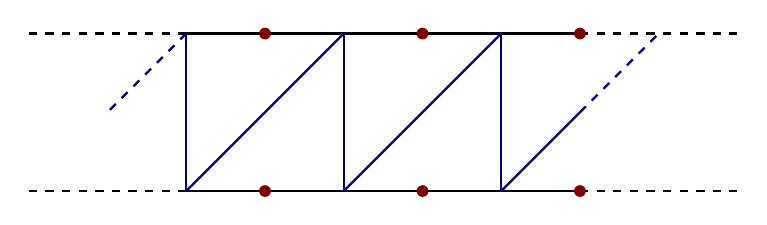
\begin{tikzpicture}
            \draw [thick] (2,2) -- (7,2);
            \draw [thick,dashed] (0,2) -- (2,2);
            \draw [thick, dashed] (7,2) -- (9,2);
            \draw [thick,dashed] (0,0) -- (2,0);
            \draw [thick,dashed] (7,0) -- (9,0);
            \draw [thick] (2,0) -- (7,0);
            \foreach \x in {3,5,7} {
                \node [circle,fill=red!50!black, inner sep=1.5pt] at (\x, 2) {};
                \node [circle,fill=red!50!black,inner sep=1.5pt] at (\x,0) {};
            }
            \draw [thick,blue!50!black] (4,0) -- (4,2);
            \draw [thick,blue!50!black] (4,0) -- (6,2);
            \draw [thick,blue!50!black] (6,2) -- (6,0);
            \draw [thick,blue!50!black] (4,2) -- (2,0);
            \draw [thick,blue!50!black] (6,0) -- (7,1);
            \draw [thick, blue!50!black,dashed] (7,1) -- (8,2);
            \draw [thick, blue!50!black] (2,0) -- (2,2);
            \draw [thick, blue!50!black, dashed] (2,2) -- (1,1);
        \end{tikzpicture}
        \caption{$\mathcal{W} (\mathbb{C}, e^z+e^{-z})$ 的生成 Lagrangian。}\label{fig:generating-Lag-equiv-P1}
    \end{figure}
    空间 $(\mathbb{C},e^z+e^{-z})$ 可如图 \ref{fig:generating-Lag-equiv-P1} 所示：红点是 $e^z+e^{-z}$ 在无穷远附近的纤维，蓝线是经指数映射 $z\mapsto e^z$ 微分同胚地投影到 $\mathbb{C}^{\ast}$ 上的 Lagrangian 子流形。我们断言，这些 Lagrangian 子流形生成包裹 Fukaya 范畴 $\mathcal{W} (\mathbb{C},e^z+e^{-z})$。\par
% [原文 p.23]
    为证明该断言，先考虑平凡 Weinstein 扇形 $X_0\coloneqq(\mathbb{C},z^2) \simeq T^{\ast} [0,1]$；此时 Weinstein 扇形 $(\mathbb{C},e^z+e^{-z})$ 可以看作把 $\mathbb{Z}$ 份 $1$-手柄按图 \ref{fig:1-handle-attaching-Z} 所示的方式粘到不交并
\[
        \bigsqcup_{\mathbb{Z}} X_0
    \]
    之上。于是显然 $\mathcal{W} (\mathbb{C},e^z+e^{-z})$ 由图 \ref{fig:1-handle-attaching-Z} 中蓝色 Lagrangian 之并生成，因为它们是扇形 $X_0$ 与各 $1$-手柄的广义余核。不难验证，这些 Lagrangian 恰好就是图 \ref{fig:generating-Lag-equiv-P1} 中所示的蓝色 Lagrangian。\par
    \begin{figure}[ht]
        \centering
        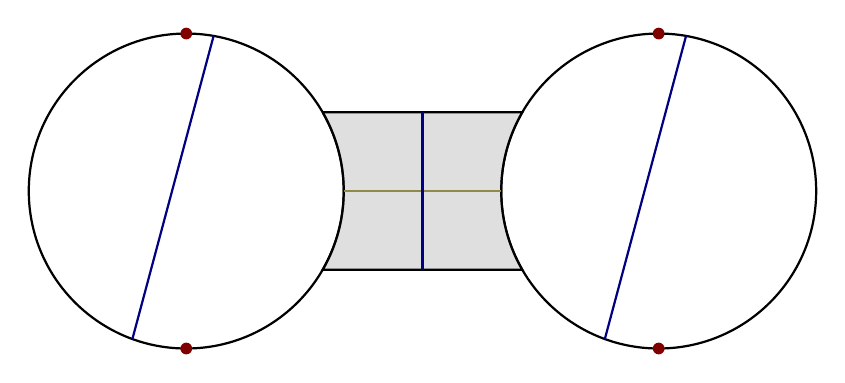
\begin{tikzpicture}
            \begin{scope}
                \draw [thick] (0,0) circle (2);
                \node [circle, fill=red!50!black, inner sep=1.5pt] at (0,2) {};
                \node [circle, fill=red!50!black, inner sep=1.5pt] at (0,-2) {};
            \end{scope}
            \begin{scope}[xshift=6cm]
                \draw [thick] (0,0) circle (2);
                \node [circle, fill=red!50!black, inner sep=1.5pt] at (0,2) {};
                \node [circle, fill=red!50!black, inner sep=1.5pt] at (0,-2) {};
            \end{scope}
            \filldraw[ fill=lightgray, fill opacity=0.5, draw=black, thick ] ({2*cos(30)},{2*sin(30)}) -- ({6+2*cos(150)},{2*sin(150)}) arc [start angle = 150, end angle = 210, radius = 2] -- ({2*cos(-30)},{2*sin(-30)}) arc [start angle = -30, end angle = 30, radius = 2];
            \draw [thick, yellow!50!black] (2,0) -- (4,0);
            \draw [thick, blue!50!black] ({2*cos(250)},{2*sin(250)}) -- ({2*cos(80)},{2*sin(80)});
            \draw [thick,blue!50!black] (3,{-2*sin(30)}) -- (3,{2*sin(30)});
            \draw [thick,blue!50!black] ({6+2*cos(250)},{2*sin(250)}) -- ({6+2*cos(80)},{2*sin(80)});
        \end{tikzpicture}
        \caption{用 $1$-手柄连接两个「标准副本」。}\label{fig:1-handle-attaching-Z}
    \end{figure}
    在计算这些 Lagrangian 的包裹 Floer 上同调之前，我们先固定一个，并把图 \ref{fig:generating-Lag-equiv-P1} 中的竖直蓝色 Lagrangian（对应图 \ref{fig:1-handle-attaching-Z} 中 $1$-手柄的余核）记作 $L_0[k]$，$k\in\mathbb{Z}$；把图 \ref{fig:generating-Lag-equiv-P1} 中的斜向 Lagrangian（对应图 \ref{fig:1-handle-attaching-Z} 中 $X_0$ 的生成 Lagrangian）记作 $L_1 [k]$。在同调镜像对称下，它们分别对应对象 $\mathcal{O}_{\mathbb{P}^1}[k]$ 与 $\mathcal{O}_{\mathbb{P}^1} (1) [k]$，其中 $k$ 是 $\mathbb{G}_m$-作用的特征。\par
    由图 \ref{fig:1-handle-attaching-Z} 显然有
\[
        CW^{\ast} (L_1[k],L_1[l])=\left\{\begin{array}{ll}
            0,&\text{若}\ l\neq k;\\
            \Bbbk,&\text{若}\ l=k.
        \end{array}\right.\quad\text{与}\quad CW^{\ast} (L_0 [k],L_0[l])=\left\{\begin{array}{ll}
            0,&\text{若}\ l\neq k;\\
            \Bbbk,&\text{若}\ l=k.
        \end{array}\right.
    \]
% [原文 p.24]
    我们约定把 $L_1[0]$ 取为 $X_0[0]$ 右侧那个 $1$-手柄里的 Lagrangian，$L_1[0]$ 就位于其中。在此约定下，同样显然有
\[
        CW^{\ast} (L_0[k],L_1 [l])=\left\{\begin{array}{ll}
            0,&\text{若}\ \vert k-l\vert\geq 2;\\
            \Bbbk,&\text{否则}.
        \end{array}\right.\quad\text{与}\quad CW^{\ast} (L_1[k],L_0[l])=0.
    \]
    于是我们完整地算出了包裹 Fukaya 范畴 $\mathcal{W} (\mathbb{C}, e^z+e^{-z})$。总结起来，$\mathcal{W} (\mathbb{C},e^z+e^{-z})$ 拟等价于无穷箭图
\[
        \begin{tikzcd}
            &\dotsb &&L_1[0] &&L_1 [1] &&\dotsb&\\
            \dotsb&&L_0[0]\arrow[ru]\arrow[lu]&&L_0[1]\arrow[ru]\arrow[lu]&&\dotsb\arrow[lu]
        \end{tikzcd}
    \]
    的路径代数上的完美模所成复形范畴。
\end{exmp}

\begin{yizhu}[特征 $k$ 的双重身份]
例中的 $k$ 同时承担两个角色：它既是 $\mathbb{Z}$-重覆盖的层数（deck 变换），又是 $\mathbb{G}_m$-作用的特征。在 B 侧它给出 $\mathcal{O}_{\mathbb{P}^1}(k)$ 的扭，在 A 侧它给出绕 $S^1$ 的单值次数，二者经同调镜像对称对应。它并不是 Floer 上同调的次数——公式里那个星号 $CW^{\ast}$ 才是同调次数，读公式时别把两者混为一谈。
\end{yizhu}
